% !TEX root = ../my-thesis.tex
%
\chapter{Introduction}
\label{sec:intro}

\cleanchapterquote{La duda es uno de los nombres de la inteligencia.}{Jorge Luis Borges}{(Argentine Writer (1899-1986))}

\section{Context: The Role of Uncertainty Quantification in Complex Engineering Systems}

Mathematical modeling is the backbone of modern engineering design and analysis. Computational models serve as the primary predictive tools used to design, verify, and ultimately certify complex engineering projects~\cite{uq_theory}. Besides its practical use, a mathematical model is also a reflection of our current level of understanding of the underlying physical phenomena. Consequently, a fundamental question arises: \textit{how do we rigorously assess the predictive fidelity of a model?}

\smallskip
The scientific method dictates that this comparison must rely on empirical validation, i.e., comparing computational predictions against physical reality. This comparison allows practitioners to evaluate whether a model accurately represents the system of interest, and crucially, to identify where and how it fails~\cite{oberkampf2010verification}. Comparing a model with empirical ground truth is also the primary mechanism for improving the model itself; it enables engineers to fine-tune parameters, adjust coefficients, or incorporate previously neglected physical behaviors. 

\smallskip
However, establishing this ground truth is not straightforward and may incur high costs. Indeed, while the ultimate verification is the operational performance of the full-scale manufactured system, relying only on late-stage prototyping is prohibitively expensive in terms of both time and financial resources. The standard alternative relies on scaled-down laboratory experiments conducted under controlled conditions. Increasingly, practitioners also rely on extremely high-fidelity computer simulations to serve as a ground truth, such as the application of \gls{dns} to assess and validate lower-fidelity turbulence models~\cite{moin1998direct}. Yet, obtaining repeatable experimental data or running scale-resolving simulations like \gls{dns} is frequently constrained by strict project budgets, schedule limitations, and immense computational costs. 

\smallskip
To mitigate these costs, a major objective in modern engineering is the development of highly reliable and cost-effective predictive models, often conceptualized as digital twins, whose capabilities can be leveraged to partially substitute physical testing during the design and certification phases. Naturally, for highly regulated and safety-critical systems, completely replacing empirical testing with computer simulations is neither feasible nor desirable~\cite{oden2010predictive}. The realistic goal is to drastically reduce the volume of required physical tests by maximizing our confidence in the computational predictions.

\smallskip
A promising research direction to achieve this confidence is provided by \gls{uq}. Because every model is ultimately a synthesis of our limited knowledge of the world~\cite{uq_theory}, \gls{uq} provides the rigorous mathematical framework necessary to systematically capture and propagate all these knowns and unknowns through the computational model. By mapping this combined uncertainty into reliable statistical confidence intervals on the simulation outputs, \gls{uq} transitions mathematical modeling from a purely deterministic estimation to a risk-informed predictive science. Ultimately, this enables engineers to make safe, optimal design decisions even when exhaustive experimental validation is out of reach.

\smallskip
Perhaps nowhere is the need for such reliable, uncertainty-aware computational modeling more pronounced than in aerospace engineering. In this field, full-scale physical testing is always financially prohibitive and time-consuming, making digital certification an attractive alternative. An example of a complex, safety-critical phenomenon that demands this level of rigorous predictive modeling is in-flight icing~\cite{Bellosta2021}.

\smallskip
In-flight icing represents one of the most critical meteorological hazards in aviation. The accretion of ice on the wings, tail, and other critical aerodynamic surfaces severely alters the flow field. This accretion leads to rapid aerodynamic performance degradation, such as increased drag and decreased lift, which can result in loss of control or catastrophic structural failure~\cite{bragg1986, Morelli2022, EASAIcing}.

\smallskip
Mitigating the risks of in-flight icing is a paramount concern for the aerospace industry. Regulatory agencies mandate rigorous certification processes to ensure that aircraft can safely operate in icing conditions. Such processes rely heavily on in-flight tests to validate the performance of anti-icing and de-icing systems. These tests are expensive, time-consuming, and often limited in scope, thus complicating the design and certification phases and inhibiting the exploration of innovative solutions. It is widely recognized that moving towards a simulation-based design paradigm and even virtual certification is essential to reduce costs, accelerate development, and enable the design of safer and more efficient aircraft~\cite{jacobi2019collection, Gori2022}.

\smallskip
Although the aerospace industry has made significant progress in the development of numerical tools for in-flight icing research, experts agree that the physics of ice accretion is complex and not yet fully understood~\cite{Guardone2025-ba}. On the one hand, we know that ice forms when water droplets in the atmosphere collide with an aerodynamic surface and, through coupled aerodynamic and thermodynamic processes, freeze and become ice. In particular, at low temperatures (usually below $-10\ \degree$C) a phenomenon known as rime ice forms, while at higher temperatures (usually between $-10\ \degree$C and $0\ \degree$C) glaze ice forms. The two types of ice have different physical characteristics and effects on the aircraft's performance, with rime ice being less dense and rougher, while glaze ice is denser and smoother~\cite{Gent2000, Caccia2023}. On the other hand, the exact mechanism that leads to ice formation is still not fully understood as it depends on a complex interplay of unknown phenomena~\cite{jacobi2019collection}, from nucleation and heat transfer on rough surfaces~\cite{Tarquini2014, kamal_2} to droplet splashing dynamics~\cite{kamal}. Furthermore, many of the parameters that govern the ice accretion process, such as droplet size, liquid water content, and ambient temperature, are subject to significant variability and uncertainty~\cite{Bellosta2021, Gori2022}. 

\smallskip
From an experimental perspective, simulating in-flight icing conditions requires the use of specialized facilities, known in the field as \textit{icing wind tunnels}. Such facilities usually consist of a wind tunnel equipped with a droplet generator and a cooling system to create the necessary conditions required by certification standards~\cite{ciraiwt, papadakis2003experimental}. However, even with these facilities, reliably simulating in-flight icing conditions is not yet possible without significant simplifications and compromises~\cite{kind1998}. The repeatability of experiments is not guaranteed even under controlled laboratory conditions, especially when dealing with glaze ice~\cite{nasa_repeatability}. 

\smallskip
From a numerical perspective, the simulation of in-flight icing is a coupled multi-physics problem that involves the computation of the flow field, droplets' trajectories and ice growth~\cite{Gori2022}. Some of the most widely used icing codes are \texttt{LEWICE}~\cite{lewice}, \texttt{FENSAP-ICE}~\cite{fensap}, \texttt{POLIMICE}~\cite{polimice}, and \texttt{IGLOO}~\cite{igloo}. All of these codes rely on a combination of empirical models, assumptions or simplifications to make the problem tractable, resulting in a significant discrepancy between the different numerical predictions and reality~\cite{many_ice_shapes, Li2023}. To further complicate the matter, the \glspl{qoi} in icing studies are often discontinuous, with abrupt transitions between different icing regimes (e.g., clean, rime, glaze, or mixed)~\cite{Gori2022, GoriGallia2024}. This discontinuous behavior poses significant challenges in the development of reliable methodologies for virtual certification, as it requires specialized techniques to accurately capture the underlying physics and ensure robust predictions.


\begin{figure}[htbp]
  \centering
  \begin{subfigure}[t]{0.49\linewidth}
       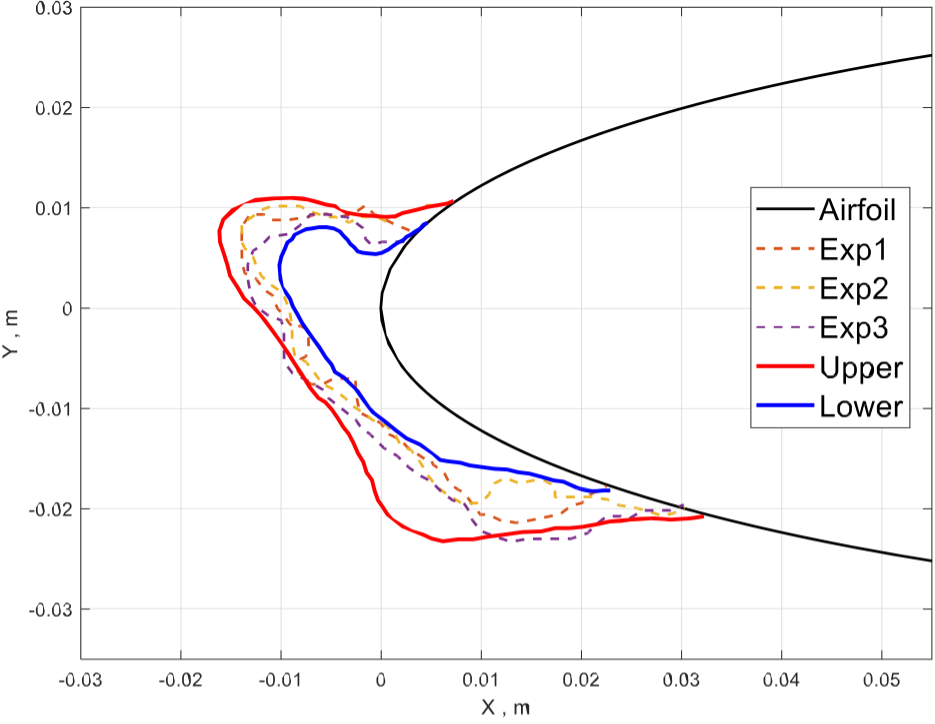
\includegraphics[width=\textwidth]{figures/intro/ice_shapes_exp.png}
    \caption{Experimental ice shapes obtained under the same conditions (3 realizations and lower and upper bounds), credits to~\cite{Li2023}.}
    \label{fig:ice_shapes_exp}
  \end{subfigure}
  \begin{subfigure}[t]{0.49\linewidth}
    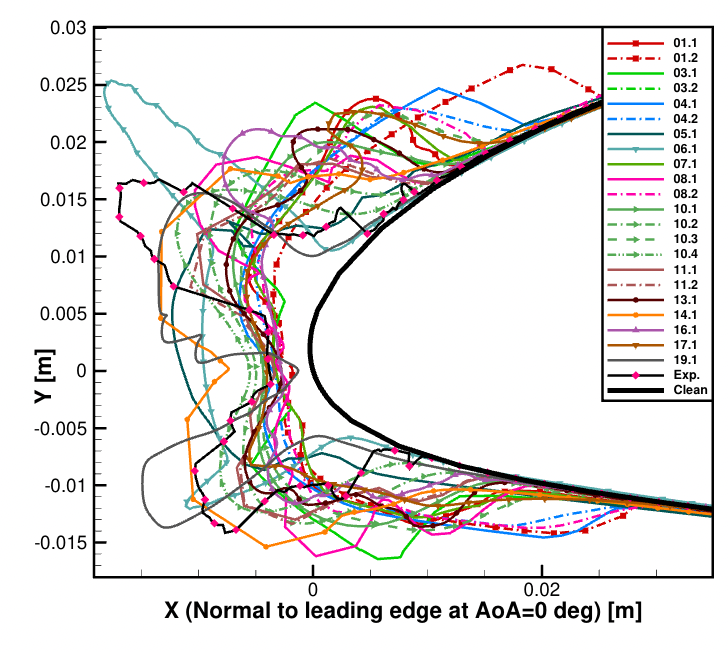
\includegraphics[width=\textwidth]{figures/intro/many_shapes_2.png}
    \caption{Numerical ice shapes obtained under the same conditions with different icing codes, credits to~\cite{many_ice_shapes_summary}.}
    \label{fig:ice_shapes_num}
  \end{subfigure}
  \caption{Experimental and numerical ice shapes' variability under the same conditions.}
  \label{fig:ice_shapes}
\end{figure}

Fig.~\ref{fig:ice_shapes} illustrates the outlined challenges in icing. Fig.~\ref{fig:ice_shapes_exp} shows the extreme variability of experimental ice shapes obtained under fixed and controlled laboratory conditions. Fig.~\ref{fig:ice_shapes_num} illustrates an even worse variability of the numerically predicted ice shapes arising from a common condition and using different codes. Together, these discrepancies demonstrate that relying on deterministic predictions or single experiments is fundamentally flawed, calling for the development of \gls{uq} methodologies capable of dealing with severe model discrepancy and noisy experimental data.

\smallskip
This PhD thesis is funded by the Marie Skłodowska-Curie Actions (MSCA) Doctoral Network TRACES (TRAining the next generation iCE researcherS)~\cite{traces}, a European initiative dedicated to advancing the predictive capability and safety metrics of in-flight icing models. While inspired by the stringent requirements of virtual certification in icing conditions, the core focus of this research is fundamentally methodological. The primary objective of this PhD thesis is to advance the core methodologies of \gls{uq} related to the development of robust numerical techniques, with a focus on reliability and precision. This is a broad and active area of scientific inquiry and research, as demonstrated by the growing number of PhD theses, see~\cite{phd1,phd3,leoni} for some very recent examples, and recently funded international collaborations, initiatives and projects, see~\cite{proj1,proj2,proj3,proj4}.

\smallskip
The main open questions in the field involve either advancing the fundamental science of statistical learning and \gls{uq}, or bridging the gap between rigorous mathematical frameworks and large-scale industrial deployment. On the fundamental side, a pervasive challenge is calibrating and tuning computer codes affected by model error, a structural discrepancy between mathematical equations and the true physical phenomena~\cite{leoni}. This un-modeled physics severely complicates the learning process, as it biases statistical learning and degrades predictive accuracy even when predicting within available data or known scenarios~\cite{uq_theory}. Looking at the icing example, it is evident that such engineering models are imperfect representations of reality, making the treatment of this discrepancy term a necessary step. Understanding and quantifying model error is only the first step; practitioners subsequently seek to use this information to classify models by their fidelity~\cite{phd3} or to optimally combine their predictions~\cite{multif}. Ultimately, leveraging the learned model error to safely extrapolate predictions or to directly correct the underlying physics of the computer code remains a profound, largely unanswered question~\cite{uq_theory}.

\smallskip
Conversely, bridging the gap between these rigorous mathematical frameworks and large-scale industrial deployment fundamentally requires mitigating the prohibitive computational burden of complex engineering pipelines. To this end, a primary enabler is the development of fast, data-driven emulators, commonly known as surrogate models~\cite{uq_theory}. However, constructing reliable emulators for realistic applications introduces severe technical hurdles, particularly the necessity to accurately capture abrupt regime changes, encompassing both true discontinuities (jumps in function values) and non-smooth physical responses (jumps in derivatives)~\cite{Sudret2023}, and scale to massive, high-dimensional output data~\cite{leoni}. Ultimately, overcoming these barriers is highly problem-specific; transitioning \gls{uq} from idealized academic test cases to industrial practice demands significant, tailored innovations within existing computational workflows.

\smallskip
Out of the open questions outlined above, this thesis chooses to investigate two specific challenges. In the first part, we address the challenge of calibrating mis-specified computer models, answering how to treat a possible model error term during the calibration phase. Answering this question will equip practitioners with a robust way to identify and quantify the model error term, paving the way to novel methodological contributions regarding its use. 

\smallskip
The second part focuses on how to reduce the computational cost associated with expensive engineering codes. Specifically, we investigate how to precisely approximate a discontinuous function with limited data and information. This contribution will overcome the poor convergence and biased predictions of standard surrogate models, unlocking practical \gls{uq} for engineering applications characterized by abrupt physical transitions.

\smallskip
These two parts are intrinsically connected. As demonstrated throughout the following chapters, computationally efficient calibration requires highly accurate surrogate models. Conversely, constructing a robust surrogate model relies heavily on an in-depth understanding of the underlying parameter space and its probabilistic structure. Having established the motivation and intrinsic connection between these two themes, we now detail the specific methodological contributions developed to address each challenge.

\section{Challenge I: Bayesian Calibration of Expensive, Mis-Specified Computer Models}
\label{sec:intro:ch1}

Before we can quantify uncertainties in numerical models, we first need to classify and understand the different sources of uncertainty; later assessing what methodologies are best suited to eliminating or mitigating them. The first class of uncertainties is \textit{aleatoric} or \textit{irreducible} uncertainty and represents inherent variability in the system or process being modeled. In the context of in-flight icing, this includes variability in atmospheric conditions such as temperature, humidity, droplet size distribution, and liquid water content~\cite{Bellosta2021}. These uncertainties cannot be reduced by gathering more knowledge and data since they are intrinsic to the system. Instead, they must be properly quantified and propagated through the models to understand their impact on predictions and decisions. The second class of uncertainties is \textit{epistemic} or \textit{reducible} uncertainty and represents a lack of knowledge about the system or process being modeled. In the context of in-flight icing, this includes uncertainties in model parameters such as the thermal conductivity of ice~\cite{ice_1, ice_2} or surface roughness~\cite{ice_3}. These uncertainties can be reduced by gathering more knowledge and data, in a process known as \textit{inference}, but they can never be completely eliminated, and thus must also be properly quantified and propagated to understand their impact on predictions and decisions~\cite{uq_theory}. In practice, inference is done by combining a numerical model of the physical process with available experimental data.

\smallskip
Treating an unknown parameter as a random quantity might seem counter-intuitive; after all, parameters such as the thermal conductivity of ice are physical constants and not random variables. If you agree with the previous statement, you are a \textit{frequentist}~\cite{fisher1925}. According to a frequentist perspective, an unknown parameter has a fixed value, and uncertainty arises only from the noise or scarcity of the data used to build an estimator of it. In contrast, a \textit{Bayesian} perspective~\cite{bayes1763} treats the unknown parameter itself as a random variable. First, a practitioner assigns a prior distribution to the parameter, which encodes beliefs about its possible values before observing any data. Then, via Bayes' theorem, the practitioner updates these beliefs with experimental data to compute a posterior distribution. Notice that the prior distribution is a subjective choice. Of course, a \textit{good} practitioner will choose a prior that is consistent with available knowledge and physical constraints. This subjective nature might seem like a weakness, but it is actually a strength, as it puts on solid philosophical grounds the idea that many decisions in engineering rely on expert knowledge. As we acquire more data, the influence of the prior distribution diminishes, and both the frequentist and Bayesian approaches converge to the same result~\cite{uq_theory, Gelman2013}. The flexibility and expressiveness of the Bayesian framework makes it particularly well-suited for complex engineering problems.

\smallskip
A very peculiar type of epistemic uncertainty is \textit{model error} or \textit{model uncertainty}, which arises from the fact that all models are the result of a series of assumptions and approximations, guided by the limited understanding of the underlying physics~\cite{fmp}. A mis-specified model will never be able to perfectly represent the data, no matter how much data we have or how well we estimate the parameters. When dealing with model error, the notion of a \textit{true} value of a parameter becomes ill-defined, as the model itself is not capable of accurately representing the underlying physical process~\cite{Plumlee2017}. In this case, the goal of inference is not to find the true value of a parameter, but rather to find a suitable pair of parameters and model error that best explains the data~\cite{uq_theory}. Although the introduction of a model error term is quite recent (in a landmark paper by Kennedy and O'Hagan~\cite{koh2001}, published in 2001), it is now widely recognized that not accounting for model error leads to biased estimates and overconfident predictions~\cite{fmp, Plumlee2017, hagan_2014}. In the context of in-flight icing, model error is believed to be a dominant source of uncertainty, especially when dealing with glaze ice or Appendix-O conditions~\cite{Bellosta2021}.

\smallskip
To this day, two main approaches have been proposed to account for model error in Bayesian calibration. The first approach, known as the \gls{fb} approach, treats both the model error and the model parameters as random variables and infers them jointly from the data~\cite{koh2001}. The \gls{fb} is the gold standard for Bayesian calibration under model uncertainty as it provides a complete and coherent treatment of the uncertainty. However, it is rarely used in practice as it increases the dimensionality of the calibration problem~\cite{fmp}. As common in engineering and mathematics, working in higher dimensional spaces opens the door to severe mathematical challenges, such as the curse of dimensionality and parameter non-identifiability, and calibration is no exception. For these reasons, practitioners usually do not treat the model error as an uncertain parameter but rather fix it to a point estimate obtained from a preliminary regression step. These approaches are known as \textit{modular}~\cite{mod_approaches}, and they allow reducing the dimensionality of the calibration problem, making it more tractable. However, as predicted by the famous \textit{No Free Lunch Theorem}~\cite{nflt}, neglecting the uncertainty in the model error term leads to biased estimates and overconfident predictions~\cite{fmp}. 

\smallskip
Consequently, a major open challenge in the field is the development of a methodology for Bayesian calibration under model error that combines the theoretical coherence of the \gls{fb} formulation with the computational tractability of modular approaches.


\section{Challenge II: Emulation of Discontinuous Responses}
\label{sec:intro:ch2}

A second fundamental challenge in the deployment of \gls{uq} is the emulation of complex computer models; that is, building cheap-to-evaluate surrogate models that can replace expensive numerical simulations.

\smallskip
Given a complex computer model, building an emulator means finding a simpler mathematical representation using a limited set of model evaluations, commonly referred to as the \gls{ndoe}. The core concept of constructing these surrogate models has deep historical roots, originating from the fundamental need to replace an \textit{expensive} function evaluation with a \textit{cheap} approximation. Naturally, the definition of \textit{expensive} has evolved alongside technology. In the 17th century, evaluating any non-polynomial function was considered prohibitively expensive because it required laborious manual calculations; the development of polynomial interpolation provided a much cheaper alternative~\cite{laplace_poly}. Two centuries later, predicting ocean tides required solving complex nonlinear \glspl{pde}, a task that demanded computational power and methodologies that did not yet exist. To bypass this bottleneck, early practitioners resorted to Fourier series and mechanical integrators to build cheap approximations of the required time series data~\cite{Tides}.


\smallskip
With the invention of digital computers and the development of numerical methods, nonlinear \glspl{pde} or complex models were no longer a computational barrier, opening the doors to a new era of scientific discovery that heavily relies on numerical simulations~\cite{uq_theory}. The notion of \textit{expensive} has evolved to refer to the fact that some tasks require multiple evaluations of a computer model. For example, optimization algorithms require hundreds or thousands of model evaluations to find the optimal solution. The work of~\cite{jones1998} introduced the use of surrogate models to reduce the computational cost associated with multiple calls to an expensive model. Even with all the advances in computational power and numerical methods, performing any rigorous \gls{uq} calculation requires millions of model calls, which is often prohibitive even for modern supercomputers~\cite{uq_theory}. For these reasons, investigations in the field of computer emulation are still an active and relevant area of research~\cite{rumsey2026}.

\smallskip
In the field of aircraft icing, numerical models are heavily based on \gls{cfd} simulations, which are notoriously expensive to run~\cite{ransles}. Due to the coupled multi-physics nature of the problem, the use of surrogate models is paramount for enabling \gls{uq} tasks such as sensitivity analysis~\cite{Bellosta2021}, and optimization~\cite{GoriGallia2024}. 

\smallskip
The holy grail of surrogate modeling is to be able to build a precise emulator using a strictly limited amount of training data. To achieve this goal, we need a high-quality \gls{ndoe} and an optimal choice of surrogate architecture. This statement aligns with the recent change in perspective within the \gls{ml} community, which has increasingly recognized that massive datasets are often less important than superior architectures~\cite{gunasekar2023textbooksneed, bettermodel, jumper2021highly}. In this context, emulating a computer model with discontinuous responses is a perfect example of a problem where the choice of architecture is far more critical than the size of the training data. Discontinuous responses are particularly challenging because abrupt transitions between different regimes can lead to poor predictions and high uncertainty. If a global surrogate model is used to replace a discontinuous computer model, two main issues arise. First, jumps lead to poor predictions in the vicinity of the discontinuity~\cite{Sudret2023}. Second, discontinuities can poison the order of convergence of the surrogate model, resulting in slower convergence rates and emulators that require significantly more training data to achieve baseline accuracy~\cite{Gori2022}. 

\smallskip
Even if global accuracy is not the primary concern, the presence of discontinuities can lead to biased parameters within the surrogate model itself. This is a special concern for \textit{interpretable} emulators, whose parameters are often used to gain insights into the underlying physics~\cite{Palar2024}. Imagine an emulator attempting to fit a function with two distinct physical regimes; the algorithm will artificially tune its parameters to find a mathematical compromise between the two, leading to non-interpretable values that do not represent either true physical state. The field of aircraft icing is particularly prone to these responses, exhibiting abrupt transitions between different icing regimes (e.g., clean, rime, glaze, or mixed). A combination of minute changes in ambient temperature, droplet size, and liquid water content can trigger a sudden transition from rime to glaze ice. Taming the impact of these discontinuous responses is therefore a mandatory component of \gls{uq} studies in this field~\cite{Gori2022, GoriGallia2024}.

\smallskip
A critical gap in the current literature is that most algorithms capable of handling discontinuous responses rely on a-priori knowledge regarding the location of the discontinuities or the exact number of physical regimes~\cite{GoriGallia2024}. More general-purpose approaches, such as~\cite{GPmixture}, require specialized sampling algorithms or careful tuning of hyperparameters, which can be unstable and time-consuming. A promising alternative relies on combining a series of well-known \gls{ml} techniques to automatically build a surrogate model that isolates discontinuous regimes~\cite{Sudret2023, Palar2024}. However, the main strength of this approach is also its fundamental weakness: it relies on a sequence of independent steps that do not inform each other, inevitably leading to sub-optimal mathematical solutions. 

\smallskip
Therefore, a pressing open challenge in surrogate modeling is the development of a unified, automated methodology capable of accurately capturing discontinuous responses without prior physical knowledge. Formulating an approach that seamlessly integrates various \gls{ml} techniques—where each step naturally and iteratively informs the next to achieve optimal predictions—remains a highly sought-after capability in modern engineering.

\section{Objectives, Contributions and Scope}
\label{sec:objectives}

Motivated by the fundamental limitations of current state-of-the-art methodologies identified in \S\ref{sec:intro:ch1} and \S\ref{sec:intro:ch2}, this work aims to answer three primary research questions:

\begin{enumerate}
  \item How can we perform Bayesian calibration under model discrepancy without incurring the prohibitive dimensionality of the \gls{fb} framework or the inherent statistical biases of modular approaches?
  \item How can we accelerate such complex calibration procedures using surrogate models without sacrificing accuracy?
  \item How can we automatically discover and accurately emulate discontinuous response surfaces in a purely data-driven manner, without relying on prior expert knowledge regarding the location or number of discontinuities?
\end{enumerate}

\smallskip
To answer these questions, the core contributions of this thesis are structured to directly resolve the open challenges previously outlined.

\smallskip
To bridge the gap between the \gls{fb} and modular paradigms, we introduce the \gls{cmp} method. As discussed in \S\ref{sec:intro:ch1}, treating model error and physical parameters jointly in a \gls{fb} framework often leads to intractable, high-dimensional calibration problems, whereas traditional modular approaches dangerously neglect model error uncertainty. The \gls{cmp} method answers this challenge by introducing a deterministic relationship between the model and model error terms, replacing the probabilistic one of the \gls{fb} framework. This effectively reduces the dimensionality of the calibration problem to that of a modular approach, but preserves the coherence and fidelity of the \gls{fb} framework.

\smallskip
While the \gls{cmp} method solves the theoretical dimensionality challenge, it introduces a new computational bottleneck: the necessity to solve an optimization problem at each sampling step. To answer the second research question and enable efficient deployment of our strategy in complex problems, we develop a novel surrogate-accelerated \gls{cmp} technique. This contribution relies on a custom-made active learning strategy that intelligently builds the representation of the model error only in areas characterized by a higher posterior probability. To demonstrate the robust applicability of calibration with model error and to test our novel calibration framework, we present a practical application to hypersonic flows. The application stems from a collaboration with the \gls{vki} (Belgium) and demonstrates the main challenges related to solving a real-world calibration problem and how to properly tackle them.

\smallskip
Finally, to tackle the discontinuity gap in surrogate modeling identified in \S\ref{sec:intro:ch2}, we propose a novel iterative piecewise emulator. Current methodologies capable of handling discontinuous regimes rely on custom-made and expensive sampling techniques. Alternatives that leverage commonly-used \gls{ml} techniques exist but are not precise enough, as they solve the problem in a series of independent steps and lead to suboptimal solutions. We answer this challenge by developing a purely data-driven algorithm that dynamically combines clustering, classification, and regression. By coupling these traditionally isolated \gls{ml} tasks into an iterative loop, each step continuously informs and refines the others. This allows the emulator to automatically partition the input space and capture abrupt physical changes without requiring any prior expert knowledge regarding the number or location of the physical regimes.

\smallskip
The scope of these contributions is primarily methodological. While fundamentally inspired by the requirements of in-flight icing, virtual certification, and aerospace engineering, this thesis establishes a general mathematical foundation in \gls{uq}. Ultimately, the methodologies developed herein are designed to unlock practical, reliable \gls{uq} for a wide range of complex, expensive, and non-smooth engineering applications.

\section{Structure of the Manuscript}
Following this introduction, Chapter~\ref{sec:ntools} provides the reader with the foundational numerical tools utilized throughout the manuscript, specifically outlining the theoretical basis of \glspl{gp}, \gls{mc} methods, and Classification with \glspl{svm}. These tools are used throughout the manuscript, and it is therefore essential to establish a common understanding of their principles and applications.

\smallskip
The manuscript is then divided into two main parts. Part I focuses on Bayesian calibration under model discrepancy, beginning with Chapter~\ref{sec:sota_1}. This chapter provides a critical review of the state-of-the-art literature, analyzing the theoretical gap between \gls{fb} and modular approaches to establish the primary motivation for the novel frameworks developed in the next chapters.

\smallskip
Chapter~\ref{sec:cmp} presents the core theoretical contribution of the first part by introducing the \gls{cmp} method. It presents the mathematical assumptions required to decouple the inference of physical parameters from model error hyperparameters, while preserving the same results as the \gls{fb} approach. The chapter also presents 4 numerical examples that demonstrate the effectiveness of the \gls{cmp} method in various scenarios.

\smallskip
To overcome the computational bottlenecks introduced by the implicit optimization of the \gls{cmp} formulation, Chapter~\ref{sec:surr} develops a surrogate-based acceleration technique. This chapter presents a novel and tailored active learning strategy that allows one to construct a surrogate model that is precise in the regions of interest, while also being computationally efficient. The chapter also presents 3 numerical examples that demonstrate the effectiveness of the surrogate-accelerated \gls{cmp} method in various scenarios.

\smallskip
Chapter~\ref{sec:cfd} transitions from methodological development to a more practical application. It demonstrates the use of the surrogate-accelerated calibration framework and more traditional ones in a hypersonic flow problem, illustrating how physically meaningful parameters can be reliably inferred despite various forms of model mis-specification and experimental errors. 

\smallskip
Part II shifts the focus toward forward uncertainty quantification and the emulation of discontinuous physical responses. Chapter~\ref{sec:sota_2} discusses existing surrogate modeling architectures, analyzing how current methods attempt to construct piecewise-continuous emulators and identifying the critical need for a generalized, algorithm-agnostic approach to detect discontinuities and partition the input space without relying on prior expert knowledge.

\smallskip
Answering this need, Chapter~\ref{sec:clustering} formalizes a purely data-driven, iterative piecewise emulation strategy. The chapter explains the mechanics of combining clustering, classification, and regression to autonomously discover the optimal spatial partitioning without requiring prior expert knowledge of the underlying regime changes or discontinuities. The chapter also presents 3 numerical examples that demonstrate the effectiveness of the proposed methodology in various scenarios of increasing dimensionality and order of discontinuity.

\smallskip
Finally, Chapter~\ref{sec:conclusion} synthesizes the outcomes of both parts, evaluating the broader impact of these methodological contributions and discussing potential future extensions and applications. 

\section{Dissemination of Research}

This thesis combines the results of multiple research activities, which have been disseminated in various forms, including peer-reviewed journal articles, presentations at international conferences, and multiple interactions with the TRACES network. Currently, the published papers are:

\begin{itemize}
    \item A paper describing the \gls{cmp} method~\cite{cmp}.
    \item A paper describing the surrogate-accelerated \gls{cmp} method~\cite{surr}.
\end{itemize}

Two contributions are currently in preparation and will be soon submitted to peer-reviewed journals:

\begin{itemize}
    \item A paper describing the calibration framework for high-enthalpy jets and its application to synthetic data, based on Chapter~\ref{sec:cfd}.
    \item A paper describing the clustering-based surrogate modeling technique for discontinuous responses, based on Chapter~\ref{sec:clustering}.
\end{itemize}

The \gls{cmp} method and the surrogate-accelerated technique were presented at the UNCECOMP 2025, the sixth edition of the International Conference on Uncertainty Quantification in Computational Science and Engineering and one of the Thematic Conferences of the European Community on Computational Methods in Applied Sciences (ECCOMAS), held in June 2025 in Rhodes, Greece.

\smallskip
The research activities were constantly presented and discussed within the TRACES network via posters, presentations, and discussions. Furthermore, calibration with model error was used during multiple research workshops of the network. Such workshops were designed to present an exercise on a virtual certification of an electro-thermal ice protection system.